%  article.tex (Version 3.3, released 19 January 2008)
%  Article to demonstrate format for SPIE Proceedings
%  Special instructions are included in this file after the
%  symbol %>>>>
%  Numerous commands are commented out, but included to show how
%  to effect various options, e.g., to print page numbers, etc.
%  This LaTeX source file is composed for LaTeX2e.

%  The following commands have been added in the SPIE class 
%  file (spie.cls) and will not be understood in other classes:
%  \supit{}, \authorinfo{}, \skiplinehalf, \keywords{}
%  The bibliography style file is called spiebib.bst, 
%  which replaces the standard style unstr.bst.  

\documentclass[]{spie}  %>>> use for US letter paper
%%\documentclass[a4paper]{spie}  %>>> use this instead for A4 paper
%%\documentclass[nocompress]{spie}  %>>> to avoid compression of citations
%% \addtolength{\voffset}{9mm}   %>>> moves text field down
%% \renewcommand{\baselinestretch}{1.65}   %>>> 1.65 for double spacing, 1.25 for 1.5 spacing 
%  The following command loads a graphics package to include images 
%  in the document. It may be necessary to specify a DVI driver option,
%  e.g., [dvips], but that may be inappropriate for some LaTeX 
%  installations. 
\usepackage[]{graphicx}
\usepackage{epstopdf}

\title{Using DARC in a Multi-Object AO Bench and in a Dome Seeing Instrument}

%>>>> The author is responsible for formatting the 
%  author list and their institutions.  Use  \skiplinehalf 
%  to separate author list from addresses and between each address.
%  The correspondence between each author and his/her address
%  can be indicated with a superscript in italics, 
%  which is easily obtained with \supit{}.

\author{Norman S\'aez$\supit{a}^{*}$, Alastair Basden\supit{b}, Dani Guzm\'an\supit{a}, Nicol\'as Dubost\supit{a}
\skiplinehalf
\supit{a}Pontificia Universidad Cat\'olica de Chile, Centre for Astro-Engineering, Av.Vicu\~na Mackenna 4860, Santiago, Chile\\
\supit{b}University of Durham, Department of Physics, Centre for Advanced Instrumentation, South Road, Durham DH1 3LE, UK\\ $*$nfsaez@uc.cl
%\supit{b}Affiliation2, Address, City, Country
}

%>>>> Further information about the authors, other than their 
%  institution and addresses, should be included as a footnote, 
%  which is facilitated by the \authorinfo{} command.

\authorinfo{Further author information: Norman S\'aez: E-mail: nfsaez@uc.cl}
%%>>>> when using amstex, you need to use @@ instead of @
 

%%%%%%%%%%%%%%%%%%%%%%%%%%%%%%%%%%%%%%%%%%%%%%%%%%%%%%%%%%%%% 
%>>>> uncomment following for page numbers
% \pagestyle{plain}    
%>>>> uncomment following to start page numbering at 301 
%\setcounter{page}{301} 
 
  \begin{document} 
  \maketitle 

%%%%%%%%%%%%%%%%%%%%%%%%%%%%%%%%%%%%%%%%%%%%%%%%%%%%%%%%%%%%% 
\begin{abstract}
The Durham adaptive Optics Real Time Controller (DARC)\cite{basden2010durham} is a real-time system
for astronomical adaptive optics systems originally developed at Durham
University and in use for the CANARY instrument. One of its main strengths is
to be a generic and high performance real-time controller running on a
off-the-shelf Linux computer. DARC is an open-source project. We are using DARC
for two different implementations: BEAGLE, a Multi-Object AO (MOAO) bench
system to experiment with novel tomographic reconstructors and LOTUCE2, an
in-dome turbulence instrument. We present the software architecture for each
application, current benchmarks and lessons learned for current and future DARC
developers.
\end{abstract}

%>>>> Include a list of keywords after the abstract 

\keywords{DARC, Adaptive Optics,  Multi-Object Adaptive Optics, real-time control, Charge Coupled Device}

%%%%%%%%%%%%%%%%%%%%%%%%%%%%%%%%%%%%%%%%%%%%%%%%%%%%%%%%%%%%%
\section{INTRODUCTION}\label{sec:intro}  % \label{} allows reference to this section
The Durham adaptive Optics Real Time Controller (DARC) is a real-time system
for astronomical adaptive optics systems originally developed at Durham
University and in use for the CANARY instrument. One of its main strengths is
to be a generic and high performance real-time controller running on a
off-the-shelf Linux computer. It was developed in a modular way making it
flexible enough to simple or sophisticated AO instruments. Very importantly,
DARC is an open-source project. Taking advantage of it modularization degree,
it is possible to implement different AO algorithms as well as different pieces
of hardware, such as cameras for wavefront sensors (WFS) and deformable
mirrors. As it is a standard Linux application, it is possible to take
advantage of external components which can be interfaced in Linux, such as
Firewire or GigE cameras. For new components, it is always possible to build a
Linux driver and Application Program Interface that can control the device.
DARC uses current multi-core technologies efficiently, performing at speeds
that were only possible to achieve with complex architectures in the past\cite{basden2012durham}. 
We are using DARC for two different implementations: BEAGLE and LOTUCE2. BEAGLE
(presented elsewhere at this conference) is a Multi-Object AO (MOAO) bench
system to experiment with novel tomographic reconstructors, such as Artificial
Neural Networks. For BEAGLE we have developed a new module within DARC, which
runs the bench in ``multiple WFS'' mode, by controlling a constellation of light
sources, three phase plates mechanisms and only one WFS camera. DARC runs this
system in conjunction with a Single Board Computer which is in charge of some
of the hardware components. LOTUCE2 (presented elsewhere at this conference) is
an in-dome turbulence instrument, which measures the angle-of-arrival of
multiple lasers to individual high-speed cameras. DARC has been used to run
four cameras, which have in-sync hardware trigger. DARC processes the pixel
streams, obtaining the angle-of-arrival from each camera, saving data to disk
and performing various analysis in real-time. We present the software
architecture for each application, current benchmarks and lessons learned for
current and future DARC developers.

\subsection{BEAGLE}
BEAGLE is a Multi-Object AO (MOAO) bench that can emulate the optical
characteristics of the William Hershel Telescope, it has two motorized phase
plates which allow change the position of the plate scale. DARC, a real-time
system for astronomical adaptive optics systems, is being used to control
acquisition images. Extra development was necessary integrate specific hardware
devices component which represents phase plate movement and guide stars. The
main features which DARC provides and BEAGLE uses are the centroid calculation
in real-time\cite{basden2012wavefront}, and camera control for Firewire
protocol. It was pending create such a way to controls new peripherals involved
to make BEAGLE works. Toward that objective, a single board computer was used.
The selected single board computer was a Beagle Bone Back (BBB). The challenge
of integrating DARC with new the single board computer was relative simple, and
relays on a local area network (TCP/IP connectivity) and scripting language
as glue. 


\subsection{LOTUCE2}
Lotuce (LOcal Turbulence Experiment)\cite{ziad1a2013lotuce} is an experimental
concept to measure and characterized the optical-turbulence inside a telescope
enclosure has been developed\cite{berdja1afirst}. LOTUCE2 is an upgraded
prototype whose main aim is to measure optical turbulence characteristics more
precisely by minimizing cross-contamination of signals. This characterization
is both quantitative (optical turbulence strength) and qualitative (assessing
        the optical turbulence statistical model). 
% in order to measure and characterize the so-called dome-seeing.


\section{Software Architecture}\label{sec:SWA} 
The Durham AO real-time controller (DARC) is composed by several software
components: The real-time control pipeline (RTCP), control, diagnostic and
graphical modules background task and scripting interface. The RTCP does main
work taking data from cameras (WFS) and computing control vectors to be send to
deformable mirrors. Control interface allows update and control RTCP, diagnostic 
module takes the output from RTCP for debug purposes.  Graphical and scripting
interfaces allows the user interact with whole system through control
interface\cite{basden2010durham}.


\subsection{BEAGLE}
BEAGLE is using DARC to control acquisition images (controlling camera with
        Firewire protocol) and centroid calculation in real-time, mainly RTCP.
Extra development was necessary integrate specific hardware devices component.
BEAGLE has to integrate phase screens movements (motors) and star guides
(stars). Toward that objective, a single board computer was used. The selected
single board computer was a Beagle Bone Back (BBB).  The challenge of
integrating DARC with new the single board computer was relative simple, and
relays on a local area network (TCP/IP connectivity) and scripting.  

Follow the same paradigms of DARC, it was installed omniORB in the BBB. This
allows develop a CORBA server, which controls most of the peripherals in the
BBB. Real time software is not required in BBB, due the way of the acquisition
methods.  For the BBB CORBA server, Python language was used. BBB has
general-purpose input/output (GPIO) which are connected to motors and leds
(phase screen and stars respectively). The BBB Server is listening requirements
to controls specific GPIO. BBB has its own python libraries to controls GPIO
called adafruit, but the performance on motors  wasn't good enough.   To
improves behaviour a  C-Python extension was developed. The extension C-Python
extension allows to use Python server importing native it, controlling GPIO
directly.

As was explained before, DARC makes possible change the system's behaviour
using scripting and control interface. BBB Server is able to communicate width
a host connected to a reachable IP address. Therefore, the communication
between DARC and BBB Server is straightforward. DARC is currently installed in a
powerful machine called RTCAOLAB, figure [\ref{fig:phy_lay}] shows the physical
layout. 
%-------------
   \begin{figure}[!ht]
   \begin{center}
   \begin{tabular}{c}
   \includegraphics[height=4.0cm]{../img/physical_layout.jpg}
   \end{tabular}
   \end{center}
   \caption[phy] 
   { \label{fig:phy_lay} BEAGLE physical layout connections}
   \end{figure} 
%-------------
Using mostly script interface, it is possible build an entire class model on
the top. RTCAOLAB was used as ``central server'', in this way, setup routines,
    calibration scripts, phase plate, stars guides are controller using only
    this host. For a user point of view, is complete transparent in which host
    is on charge of which device. Figure [\ref{fig:class}] shows the complete class
    model build on the top.

%-------------
   \begin{figure}[!ht]
   \begin{center}
   \begin{tabular}{c}
   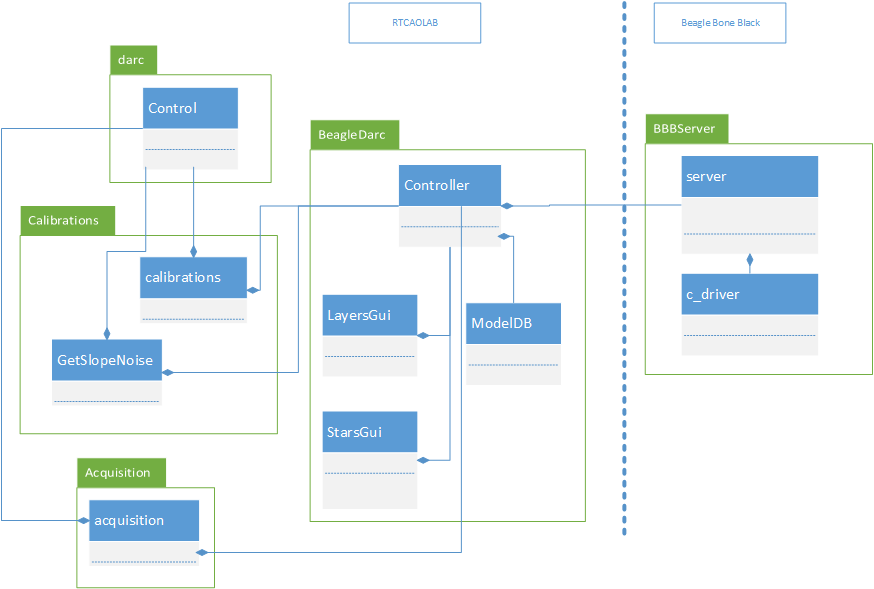
\includegraphics[height=9.0cm]{../img/class_model2.png}
   \end{tabular}
   \end{center}
   \caption[class] 
   { \label{fig:class} BeagleDarc Class Model. White boxes contains host name where those packages are deployed.}
   \end{figure}
%-------------
\subsection{LOTUCE2}
Lotuce (LOcal Turbulence Experiment) is an experimental to measure and
characterized the optical-turbulence inside a telescope enclosure. LOTUCE2 is
an upgraded prototype whose main aim is to measure optical turbulence
characteristics more precisely by minimizing cross-contamination of signals.
Initially, Lotuce used a single camera, LOTUCE2 instead  uses four cameras. The
core functionality being used by LOTUCE2 and camera acquisition and slope
calculation, all provided by DARC.  

Replicate a software environment was an item to be worry about. In order to
make confident enough that it is possible replicate the environment, DARC was
installed in two different machines. Mac Book pro Late2011 and Desktop machine
were the host for DARC current deployment. Different operative system were used,
     but the same software were compiled over them. Desktop machine were used a
     Fedora 14 Linux kernel 2.6.35.13-91 32 bits architecture. Mac Book pro
     instead has installed a Linux Ubuntu 13.10 kernel 3.11.0-15 64 bits
     architecture.  Besides this difference, the behaviour was exactly the
     same. Notice that each kernel is not patched as real time, but is was good
     enough for LOTUCE2 purposes.

DARC is highly flexible with each camera protocol, it can handle USB, iee1394
cameras (fire-wire cameras) as well as Ethernet Gig protocols. Cameras used are
two Gigabit Ethernet protocol, Cisco 3560 was configured to plug all possible
cameras. This switch was transparent for DARC for either installation.  

Camera synchronization were a defiance to face. The approach taken was an
external trigger shared among the cameras. The device used to trigger the
camera acquisition is a single board computer, integrated and configurable
GPIO.  Beagle Bone Black (BBB) was the selected one for these purposes. BBB has
an ARM Cortex-A8 processor, with a Linux inside. BBB uses an embedded Ubuntu
13.10 Linux . 100 [KHz] is the  maximum frequency reached turning on off a
GPIO. To improve this situation, a programmable real-time unit(PRU) was used.
This unit performs embedded tasks that require real-time constraints. PRU is a
subsystem of the processor inside BBB. It is an independent CPU with its own
memory and instruction set. It can run its own program, completely independent
of the Linux kernel on the main CPU. Using PRU approach BBB could reach a
signal frequency of 200[MHz], accomplishing  with LOTUCE22 requirements.  

DARC can get both camera data in a single stream or each camera in a separated
stream. If a single stream approach is used, the streams a stick one next to
the other. It is mandatory that each camera protocol has its own driver
implementation make it compatible with DARC. Aravis is a library for video
acquisition which are being used to make the driver work in DARC. Preliminary
shows promising results, frames per seconds for our purposes should be up to
125. Using both cameras at same time (but not at maximum resolution) we are
getting results up to 200fps.  The trigger to acquire an image with cameras is
working fine but is still under testing. See figure [\ref{fig:lpl}] that shows the
current layout design. Slight modifications are not discard at this time.  
%-------------
   \begin{figure}[!ht]
   \begin{center}
   \begin{tabular}{c}
   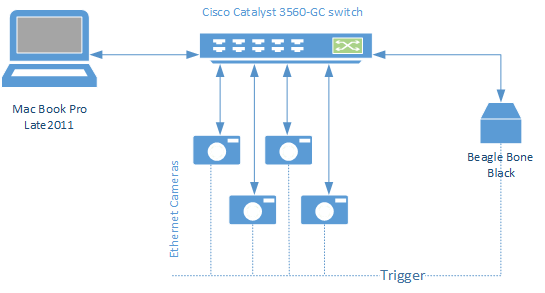
\includegraphics[height=6.0cm]{../img/physical_layout_lotuce.png}
   \end{tabular}
   \end{center}
   \caption[lpl] 
   { \label{fig:lpl} LOTUCE2 physical layout}
   \end{figure} 
%-------------

The main program should be running where DARC is installed (either Mac Book pro
        or Desktop) and the signal trigger it will be send using TCP/IP
protocol, arriving at BBB, triggering the acquisition. Some automatic routines
are being implemented, like automatic sub aperture location, ideal image size
and some graphics plots to help to controls the instrument operations. Image
[\ref{fig:step2}] shows a prototype GUI example.

%-------------
   \begin{figure}[!ht]
   \begin{center}
   \begin{tabular}{c}
   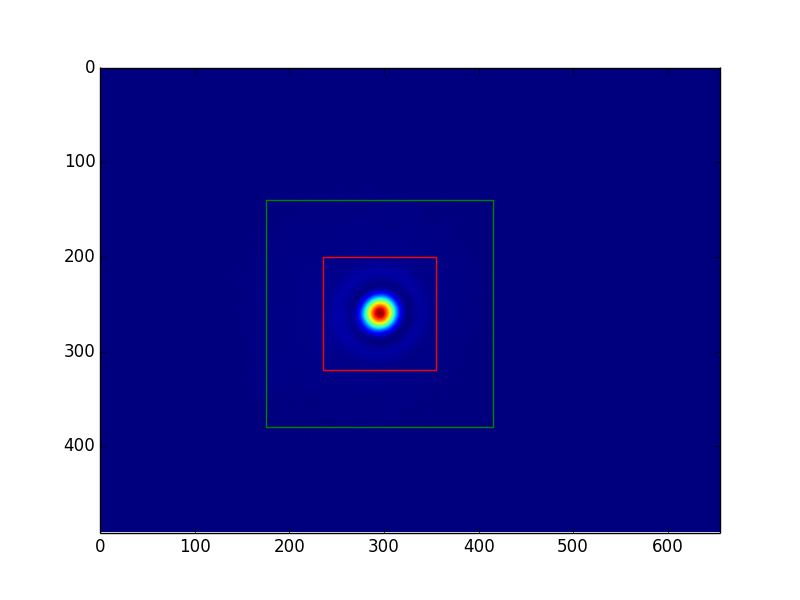
\includegraphics[height=6.0cm]{../img/step2b.png}
   \end{tabular}
   \end{center}
   \caption[step2] 
   { \label{fig:step2} LOTUCE2 after adjust sub aperture location (red) and image size (green)}
   \end{figure} 
%-------------

Most of the modules and interfaces are still under development.
%%%%%%%%%%%%%%%%%%%%%%%%%%%%%%%%%%%%%%%%%%%%%%%%%%%%%%%%%%%%%
\section{Software Development and Experimental Tests Experience} \label{sec:LL}
This section belongs to software development that were implemented, and
experimental test involved BEAGLE and LOTUCE2. 
\subsection{BEAGLE}
Most of the current work has been implemented using DARC CORBA control
interface. This allows quick prototype of calibration functions to setup the
bench. As is showed in [\ref{fig:class}] classes over 
\subsection{LOTUCE2}



%\newpage
%\section{Conclusions}

%\appendix    %>>>> this command starts appendixes
%%%%%%%%%%%%%%%%%%%%%%%%%%%%%%%%%%%%%%%%%%%%%%%%%%%%
%%%%%%%%%%%%%%%%%%%%%%%%%%%%%%%%%%%%%%%%%%%%%%%%%%%%%%%%%%%%%
%\acknowledgments     %>>>> equivalent to \section*{ACKNOWLEDGMENTS}       
 
%[...]

%%%%%%%%%%%%%%%%%%%%%%%%%%%%%%%%%%%%%%%%%%%%%%%%%%%%%%%%%%%%%
%%%%% References %%%%%

\newpage
\acknowledgments{Hi}
\bibliography{report}   %>>>> bibliography data in report.bib
\bibliographystyle{spiebib}   %>>>> makes bibtex use spiebib.bst

\end{document} 
